\begin{ZhChapter}

\chapter{Proposed Algorithm}
In this chapter, we will introduce the architecture and flowchart of our algorithm. Next, we will provide an in-depth explanation of our proposed algorithm, including the underlying concepts and the rationale behind our approach. Subsequently, we will present a detailed description of our software and hardware specifications, as well as the setup procedures. Finally, we will execute the experiment and describe how we implemented our concept and successfully completed the entire experiment.
\section{Main Method} %Chapter 3.1
Figure \ref{fig: softwareStack} illustrates our software stack. On our existing hardware, we use Windows 11 as our operating system. In addition, we use Python 3.9.18 as the programming language for this research. Based on Python 3.9.18, the main packages we use are TensorFlow, NumPy, and Scikit-learn.
\begin{figure*}[htbp]
    \centering
    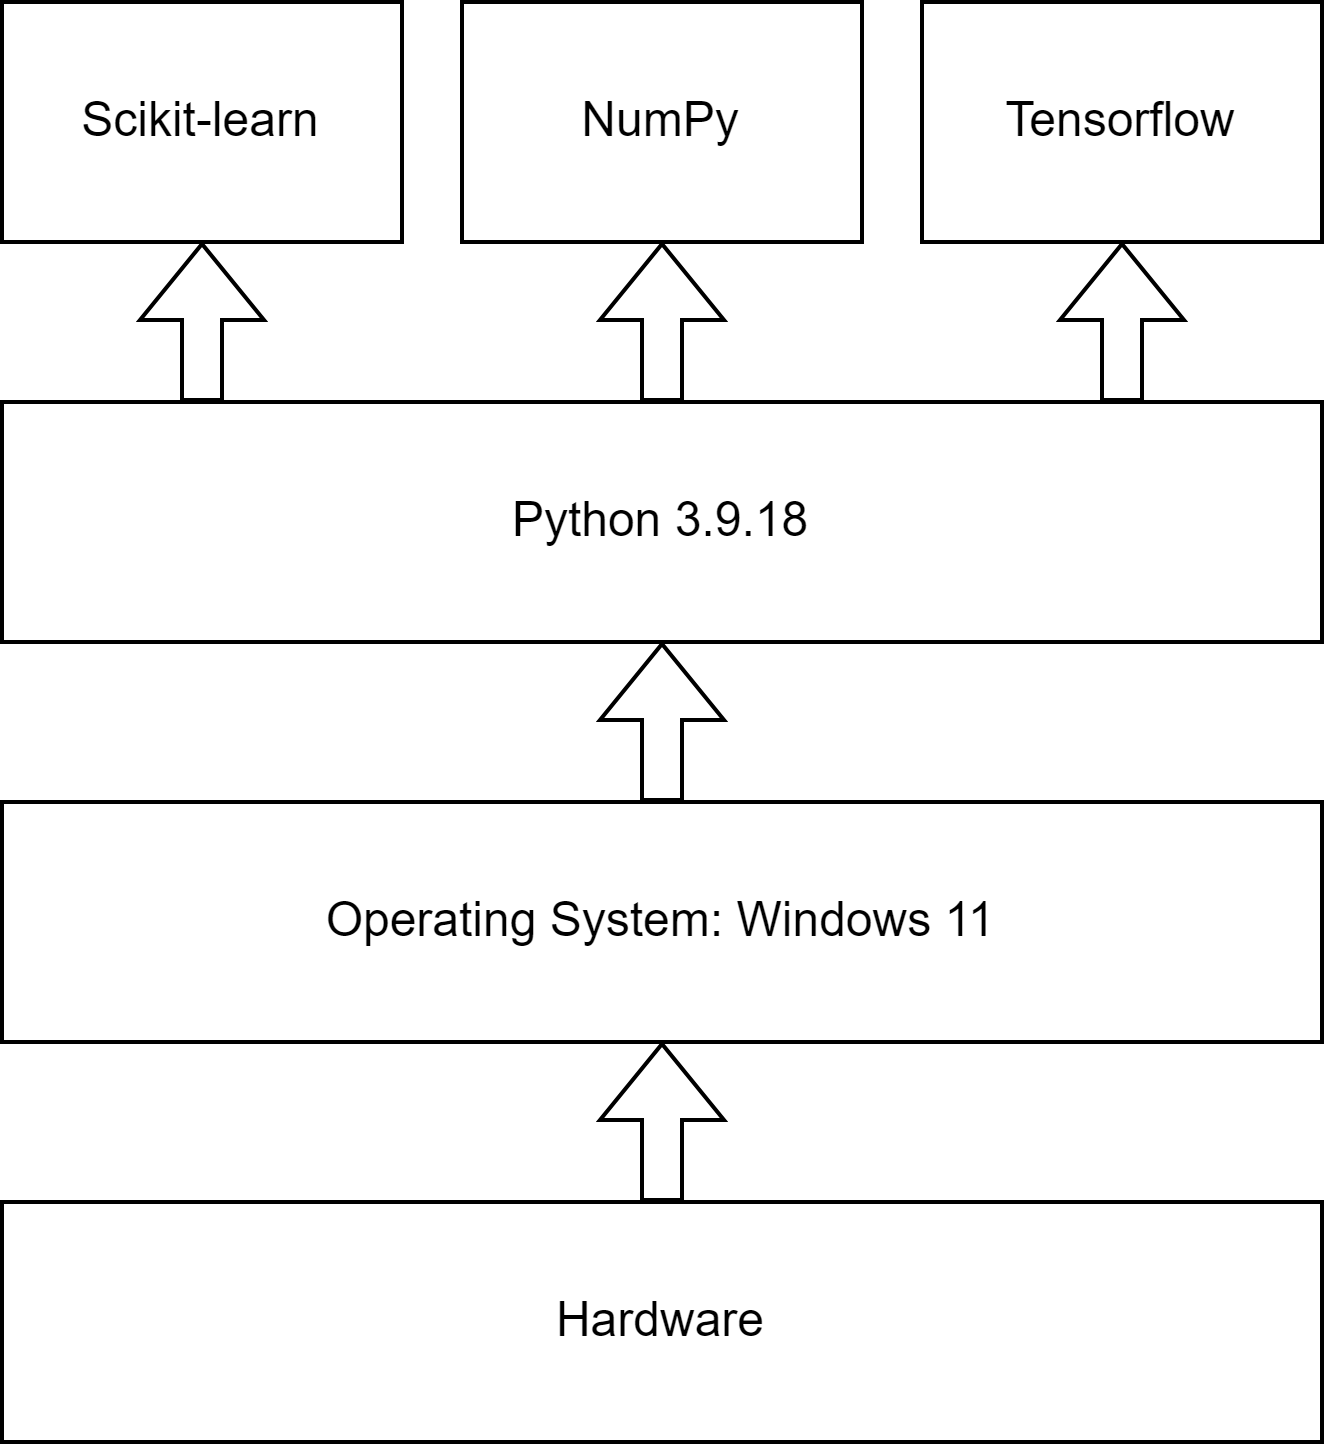
\includegraphics[width = 0.75\textwidth]{image/softwareStack.png}
    \caption{Software stack for Efficiency-based GP}
    \label{fig: softwareStack}
\end{figure*}

In previous research \cite{akhmedova2024generationlossfunctionimage}, we observed that genetic operations are performed on the entire population, requiring the evaluation of the entire new population after each complete set of genetic operations. However, the evaluation process is time-consuming. Therefore, in this study, we will employ the concept of a sample tournament to select certain individuals rather than the entire population for genetic operations. By doing so, we only need to evaluate the newly generated individuals. Figure \ref{fig: FlowChart} illustrates the conceptual flowchart of this study.

As illustrated in the figure \ref{fig: FlowChart}, we initialize a population consisting of $P$ individuals before commencing the experiment. Once initialized, we evaluate all individuals, store their scores, and identify the best score for subsequent analysis and research. The process then enters a loop, continuing until the generation number reaches the specified value. Initially in this loop, we use a sample tournament to randomly select $N$ individuals from the population, followed by choosing the top $X$ individuals for genetic operations (crossover and mutation). The offspring of these $X$ individuals are then evaluated and added to the population. We update the best-performing individual and remove the poorly performing individuals until the population size returns to $P$. Upon concluding the loop, we generate the best-performing loss function and conclude the experiment.

\begin{figure*}[htbp]
    \centering
    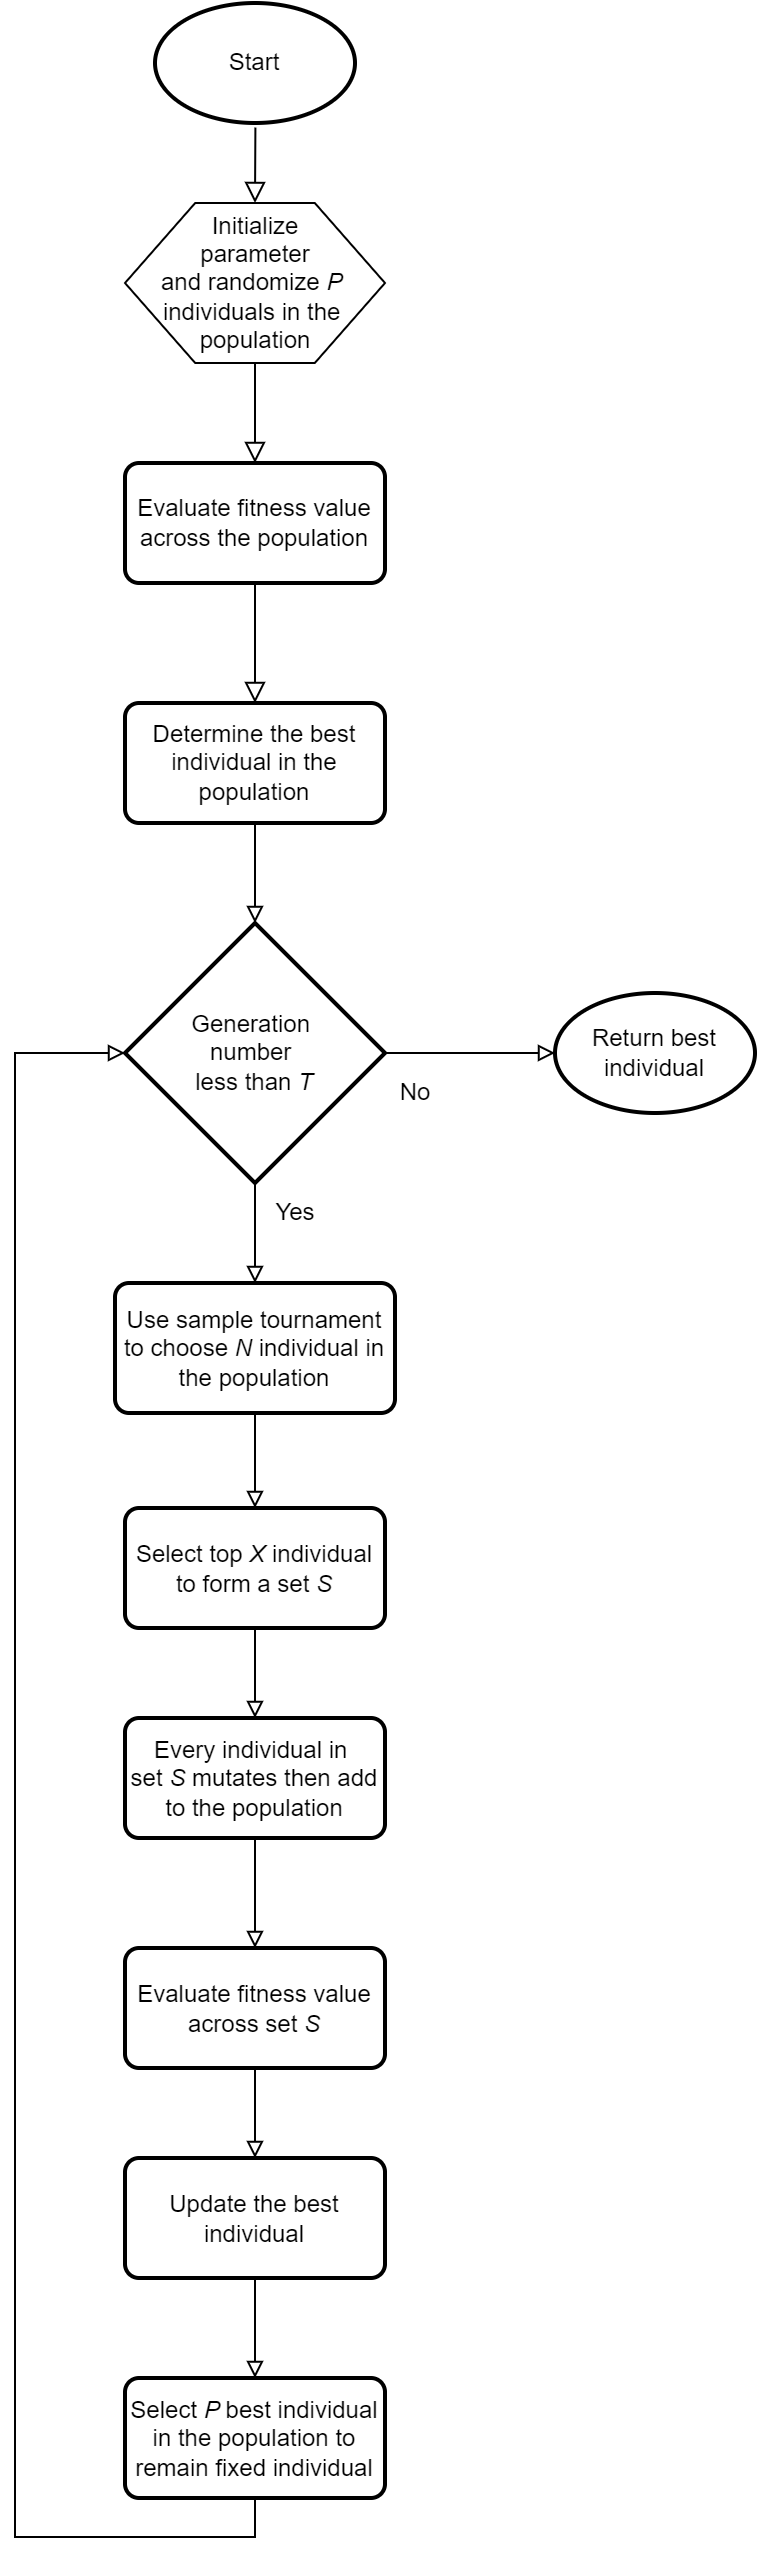
\includegraphics[width = 1\textwidth]{image/FlowChart.png}
    \caption{FlowChart for Efficiency-based GP}
    \label{fig: FlowChart}
\end{figure*}

\section{Implementation Details}
To implement our experiment, the hardware and software requirements are first defined in Section 3.2.1. Next, the environment setup steps are described in Section 3.2.2. Finally, the implementation steps are explained in Section 3.2.3.
\subsection{Requirements}

Table \ref{tab: softwareSpec} outlines our software requirements. Our code execution environment is Windows 11. We utilize Python version 3.9.18 and TensorFlow version 2.6.0. The specific packages used within Python and TensorFlow are detailed in Table \ref{tab: packageSpec}.

\begin{table*}[htbp]
\centering
\caption{Software requirements} \label{tab: softwareSpec}
\makebox[\linewidth][c]{
    \renewcommand\arraystretch{1.2}{
        \begin{tabular}{| l | c  c |}
        \hline
        Software Type & Software Name & Version \\
        \hline
        Operating System & Windows &  11 \\
        Programming Language & Python & 3.9.18\\
        \hline
        \end {tabular}
    }}
\end {table*}

\begin{table*}[htbp]
\centering
\caption{Python package requirements} \label{tab: packageSpec}
\makebox[\linewidth][c]{
    \renewcommand\arraystretch{1.2}{
        \begin{tabular}{| l | c  c |}
        \hline
        Package Name/Version & Imported from & License \\
        \hline
        tensorflow/2.6.0 & N/A & Apache License 2.0\\
        numpy/1.20.3 & N/A & modified BSD license\\
        cudnn/8.2.1 & N/A & N/A\\
        os & N/A & N/A\\
        copy  & N/A & N/A\\
        time  & N/A & N/A\\
        math  & N/A & N/A\\
        random & N/A & N/A\\
        datetime & datetime & N/A\\
        cmp\_to\_key & functools & N/A\\
        Sequential & tensorflow.keras.models & N/A\\
        Dense & tensorflow.keras.layers & N/A\\
        Flatten & tensorflow.keras.layers & N/A\\
        Dropout & tensorflow.keras.layers & N/A\\
        UpSampling2D & tensorflow.keras.layers & N/A\\
        BatchNormalization & tensorflow.keras.layers & N/A\\
        InceptionV3 & tensorflow.keras.applications.inception\_v3 & N/A\\
        preprocess\_input & tensorflow.keras.applications.inception\_v3 & N/A\\
        ReduceLROnPlateau & tensorflow.keras.callbacks & N/A\\
        to\_categorical & tensorflow.keras.utils & N/A\\
        train\_test\_split/1.5.2 & sklearn.model\_selection & N/A\\
        ImageDataGenerator & tensorflow.keras.preprocessing.image & N/A\\
        np\_config & tensorflow.python.ops.numpy\_ops & N/A\\
        \hline
        \end {tabular}
    }}
\end {table*}

Table \ref{tab: hardwareSpec} presents our hardware requirements. The computer we used to execute our code is equipped with a 13th Gen Intel(R) Core(TM) i7-13700 CPU, 32GB of memory operating at a frequency of DDR5-5600MHz, and an NVIDIA GeForce RTX 4060 GPU to meet our computational needs.

\begin{table*}[htbp]
\centering
\caption{Hardware requirements} \label{tab: hardwareSpec}
\makebox[\linewidth][c]{
    \renewcommand\arraystretch{1.2}{
        \begin{tabular}{| l | c |}
        \hline
        Hardware Type & Name \\
        \hline
        CPU & 13th Gen Intel(R) Core(TM) i7-13700 \\
        Memory & DDR5-5600MHz 32 GB \\
        Graphic Card & NVIDIA GeForce RTX 4060 \\
        \hline
        \end {tabular}
    }}
\end {table*}

\subsection{Environment Setup}

The following section will describe how to properly set up the environment we used to conduct our experiment. First, we used Anaconda as our package management tool for the implementation. Therefore, you must first visit the Anaconda official website (\url{https://www.anaconda.com/download}) to download the software. As shown in figure \ref{fig: conda}, click the Download button to complete the download.

\begin{figure*}[htbp]
    \centering
    
\includegraphics[width = 0.75\textwidth]{image/conda.jpg}
    \caption{Anaconda official website}
    \label{fig: conda}
\end{figure*}

After installation, we need to create a new environment to ensure the independence of all the packages. In Anaconda prompt, enter \verb|conda create --name environment-name| to create a new environment, as shown in figure \ref{fig: createEnv}. Next, enter \verb|conda activate environment-name| to activate the environment just like the first prompt entered in figure \ref{fig: tensorflow}.

\begin{figure*}[htbp]
    \centering
    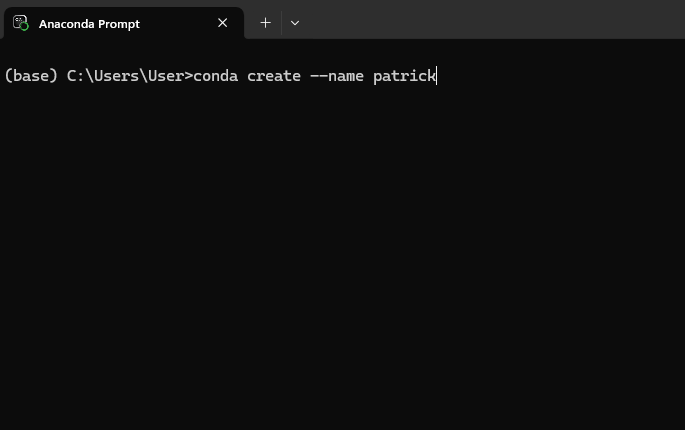
\includegraphics[width = 0.75\textwidth]{image/createEnv.png}
    \caption{Conda prompt for creating new environment}
    \label{fig: createEnv}
\end{figure*}

Since directly installing TensorFlow may result in the installation of incompatible versions of NumPy, we first use the command shown in figure \ref{fig: numpy} to download version 1.20.3 of  NumPy: \verb|conda install numpy=1.20|. Afterward, we can install the GPU version of TensorFlow by entering the following command in the Anaconda prompt: \verb|conda install tensorflow-gpu|, as shown in figure \ref{fig: tensorflow}. Finally, we need to download Scikit-learn to split the dataset during the model training process. As shown in figure \ref{fig: sklearn}, enter the following command to complete the final installation step: \verb|conda install scikit-learn|.

\begin{figure*}[htbp]
    \centering
    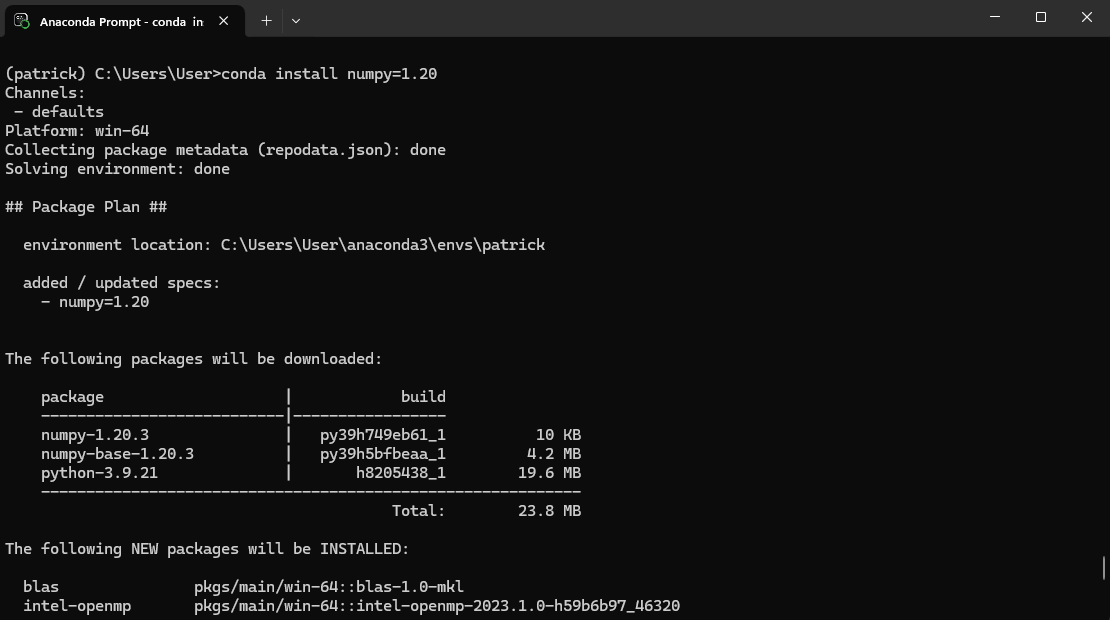
\includegraphics[width = 0.75\textwidth]{image/numpy.png}
    \caption{Install numpy in conda environment}
    \label{fig: numpy}
\end{figure*}

\begin{figure*}[htbp]
    \centering
    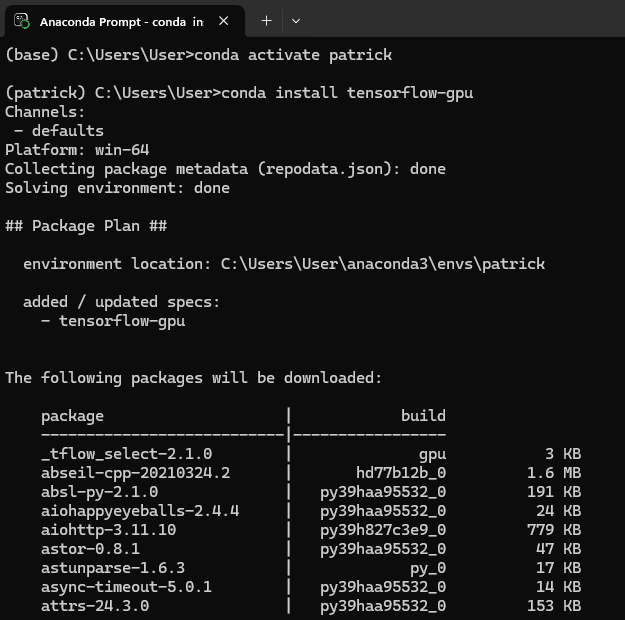
\includegraphics[width = 0.75\textwidth]{image/tensorflow.png}
    \caption{Install tensorflow in conda environment}
    \label{fig: tensorflow}
\end{figure*}

\begin{figure*}[htbp]
    \centering
    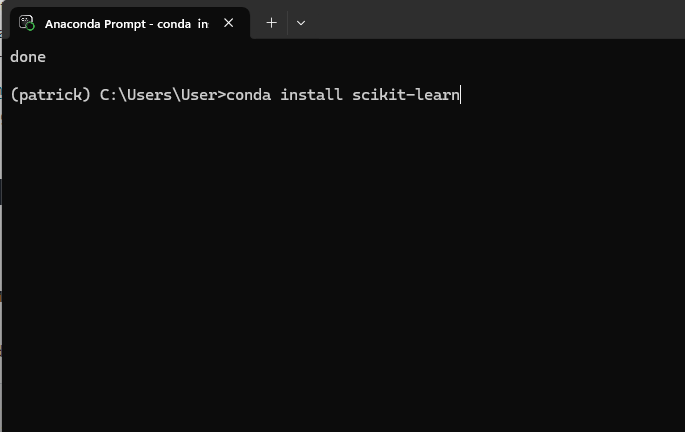
\includegraphics[width = 0.75\textwidth]{image/sklearn.png}
    \caption{Install scikit-learn in conda environment}
    \label{fig: sklearn}
\end{figure*}

\subsection{Implementation Steps}
Based on the architecture we introduced on section 3.1, the pseudo code of this algorithm is presented as below.
\begin{algorithm}
    \caption{Efficiency-based GP to generate loss function}\label{alg:cap}
    \begin{algorithmic}
        \State Initialize: \space $P = \space 8$, $T =\space 12$, $G =\space P*3/4$, $N = \space G/2$, $C_r = \space0.5$, $M_{ST} = \space0.3$, $M_N = \space0.1$
        \State Randomly initialize population which include P trees
        \State Evaluate GP fitness function $F$ for each individual in the population
        \State Determine the best individual
        \While{generation number < $T$}
        \State $S$ = Sample tournament G $\sim$ Uniform (P)
        \State Select top $N$ trees from $G$ to form a set $S$
        \For{Individual in $S$}
        \If {$rand_1 < 0.5$}
        \State random\_individual = Randomly select a individual in $S$ except Individual
        \Else
        \State random\_individual = Randomly generated tree
        \EndIf
        \State generated\_child = Crossover(Individual, random\_individual)
        \If {$rand_2 < M_{ST}$}
        \State Apply subtree mutation to the generated\_child
        \EndIf
        \If {$rand_3 < M_N$}
        \State Apply one-point mutation to the generated\_child
        \EndIf
        \EndFor
        \State Evaluated GP fitness function $F$ for each generated child individual
        \State Update the best individual
        \State Select $P$ best trees from population to form a new population containing $P$ trees
        \EndWhile
    \end{algorithmic}
\end{algorithm}

\end{ZhChapter}